\documentclass{standalone}
\usepackage{pgfplots}
\usepackage{pgfplotstable}
\pgfplotsset{compat=1.16}
\usetikzlibrary{matrix,chains,trees,scopes,decorations,arrows.meta,automata,positioning,shadows,3d}


\begin{document}
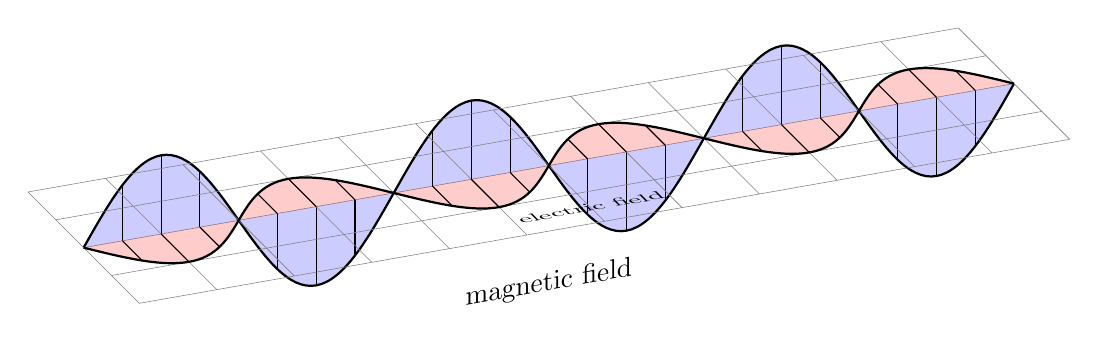
\begin{tikzpicture}[z={(10:10mm)},x={(-45:5mm)}]
    \def\wave{
    \draw[fill,thick,fill opacity=.2]
    (0,0) sin (1,1) cos (2,0) sin (3,-1) cos (4,0)
    sin (5,1) cos (6,0) sin (7,-1) cos (8,0)
    sin (9,1) cos (10,0)sin (11,-1)cos (12,0);
    \foreach \shift in {0,4,8}
    {
    \begin{scope}[xshift=\shift cm,thin]
    \draw (.5,0) -- (0.5,0 |- 45:1cm);
    \draw (1,0) -- (1,1);
    \draw (1.5,0) -- (1.5,0 |- 45:1cm);
    \draw (2.5,0) -- (2.5,0 |- -45:1cm);
    \draw (3,0) -- (3,-1);
    \draw (3.5,0) -- (3.5,0 |- -45:1cm);
    \end{scope}
    }
    }
    \begin{scope}[canvas is zy plane at x=0,fill=blue]
    \wave
    \node at (6,-1.5) [transform shape] {magnetic field};
    \end{scope}
    \begin{scope}[canvas is zx plane at y=0,fill=red]
    \draw[help lines] (0,-2) grid (12,2);
    \wave
    \node at (6,1.5) [rotate=180,xscale=-1,transform shape] {electric field};
    \end{scope}
\end{tikzpicture}
\end{document}